% This file is generated by the MATLAB m-file laprint.m. It can be included
% into LaTeX documents using the packages graphicx, color and psfrag.
% It is accompanied by a postscript file. A sample LaTeX file is:
%    \documentclass{article}\usepackage{graphicx,color,psfrag}
%    \begin{document}% This file is generated by the MATLAB m-file laprint.m. It can be included
% into LaTeX documents using the packages graphicx, color and psfrag.
% It is accompanied by a postscript file. A sample LaTeX file is:
%    \documentclass{article}\usepackage{graphicx,color,psfrag}
%    \begin{document}% This file is generated by the MATLAB m-file laprint.m. It can be included
% into LaTeX documents using the packages graphicx, color and psfrag.
% It is accompanied by a postscript file. A sample LaTeX file is:
%    \documentclass{article}\usepackage{graphicx,color,psfrag}
%    \begin{document}% This file is generated by the MATLAB m-file laprint.m. It can be included
% into LaTeX documents using the packages graphicx, color and psfrag.
% It is accompanied by a postscript file. A sample LaTeX file is:
%    \documentclass{article}\usepackage{graphicx,color,psfrag}
%    \begin{document}\input{bias_sigma_1_85}\end{document}
% See http://www.mathworks.de/matlabcentral/fileexchange/loadFile.do?objectId=4638
% for recent versions of laprint.m.
%
% created by:           LaPrint version 3.16 (13.9.2004)
% created on:           16-Jul-2013 16:48:36
% eps bounding box:     15 cm x 11.25 cm
% comment:              
%
\begin{psfrags}%
\psfragscanon%
%
% text strings:
\psfrag{s03}[t][t]{\color[rgb]{0,0,0}\setlength{\tabcolsep}{0pt}\begin{tabular}{c}{\Large{}Calculation number}\end{tabular}}%
\psfrag{s04}[b][b]{\color[rgb]{0,0,0}\setlength{\tabcolsep}{0pt}\begin{tabular}{c}{\Large$\log \sigma_1$}\end{tabular}}%
%
% xticklabels:
\psfrag{x01}[t][t]{1}%
\psfrag{x02}[t][t]{2}%
\psfrag{x03}[t][t]{3}%
\psfrag{x04}[t][t]{4}%
\psfrag{x05}[t][t]{5}%
\psfrag{x06}[t][t]{6}%
\psfrag{x07}[t][t]{7}%
\psfrag{x08}[t][t]{8}%
\psfrag{x09}[t][t]{9}%
\psfrag{x10}[t][t]{10}%
\psfrag{x11}[t][t]{11}%
\psfrag{x12}[t][t]{12}%
\psfrag{x13}[t][t]{13}%
\psfrag{x14}[t][t]{14}%
\psfrag{x15}[t][t]{15}%
\psfrag{x16}[t][t]{16}%
\psfrag{x17}[t][t]{17}%
\psfrag{x18}[t][t]{18}%
\psfrag{x19}[t][t]{19}%
\psfrag{x20}[t][t]{20}%
%
% yticklabels:
\psfrag{v01}[r][r]{-5.9}%
\psfrag{v02}[r][r]{-5.8}%
\psfrag{v03}[r][r]{-5.7}%
\psfrag{v04}[r][r]{-5.6}%
\psfrag{v05}[r][r]{-5.5}%
\psfrag{v06}[r][r]{-5.4}%
\psfrag{v07}[r][r]{-5.3}%
\psfrag{v08}[r][r]{-5.2}%
\psfrag{v09}[r][r]{-5.1}%
\psfrag{v10}[r][r]{-5}%
\psfrag{v11}[r][r]{-4.9}%
%
% Figure:
\resizebox{12cm}{!}{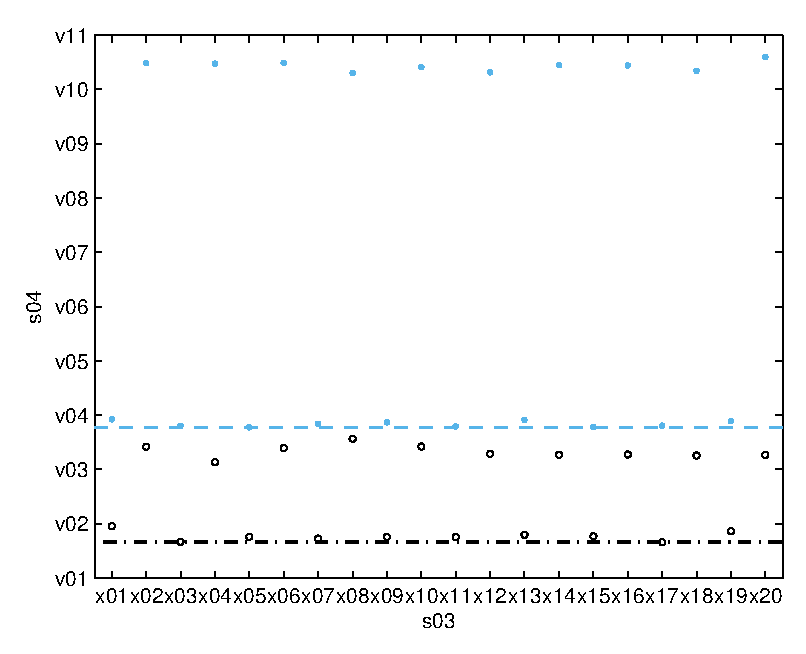
\includegraphics{bias_sigma_1_85.eps}}%
\end{psfrags}%
%
% End bias_sigma_1_85.tex
\end{document}
% See http://www.mathworks.de/matlabcentral/fileexchange/loadFile.do?objectId=4638
% for recent versions of laprint.m.
%
% created by:           LaPrint version 3.16 (13.9.2004)
% created on:           16-Jul-2013 16:48:36
% eps bounding box:     15 cm x 11.25 cm
% comment:              
%
\begin{psfrags}%
\psfragscanon%
%
% text strings:
\psfrag{s03}[t][t]{\color[rgb]{0,0,0}\setlength{\tabcolsep}{0pt}\begin{tabular}{c}{\Large{}Calculation number}\end{tabular}}%
\psfrag{s04}[b][b]{\color[rgb]{0,0,0}\setlength{\tabcolsep}{0pt}\begin{tabular}{c}{\Large$\log \sigma_1$}\end{tabular}}%
%
% xticklabels:
\psfrag{x01}[t][t]{1}%
\psfrag{x02}[t][t]{2}%
\psfrag{x03}[t][t]{3}%
\psfrag{x04}[t][t]{4}%
\psfrag{x05}[t][t]{5}%
\psfrag{x06}[t][t]{6}%
\psfrag{x07}[t][t]{7}%
\psfrag{x08}[t][t]{8}%
\psfrag{x09}[t][t]{9}%
\psfrag{x10}[t][t]{10}%
\psfrag{x11}[t][t]{11}%
\psfrag{x12}[t][t]{12}%
\psfrag{x13}[t][t]{13}%
\psfrag{x14}[t][t]{14}%
\psfrag{x15}[t][t]{15}%
\psfrag{x16}[t][t]{16}%
\psfrag{x17}[t][t]{17}%
\psfrag{x18}[t][t]{18}%
\psfrag{x19}[t][t]{19}%
\psfrag{x20}[t][t]{20}%
%
% yticklabels:
\psfrag{v01}[r][r]{-5.9}%
\psfrag{v02}[r][r]{-5.8}%
\psfrag{v03}[r][r]{-5.7}%
\psfrag{v04}[r][r]{-5.6}%
\psfrag{v05}[r][r]{-5.5}%
\psfrag{v06}[r][r]{-5.4}%
\psfrag{v07}[r][r]{-5.3}%
\psfrag{v08}[r][r]{-5.2}%
\psfrag{v09}[r][r]{-5.1}%
\psfrag{v10}[r][r]{-5}%
\psfrag{v11}[r][r]{-4.9}%
%
% Figure:
\resizebox{12cm}{!}{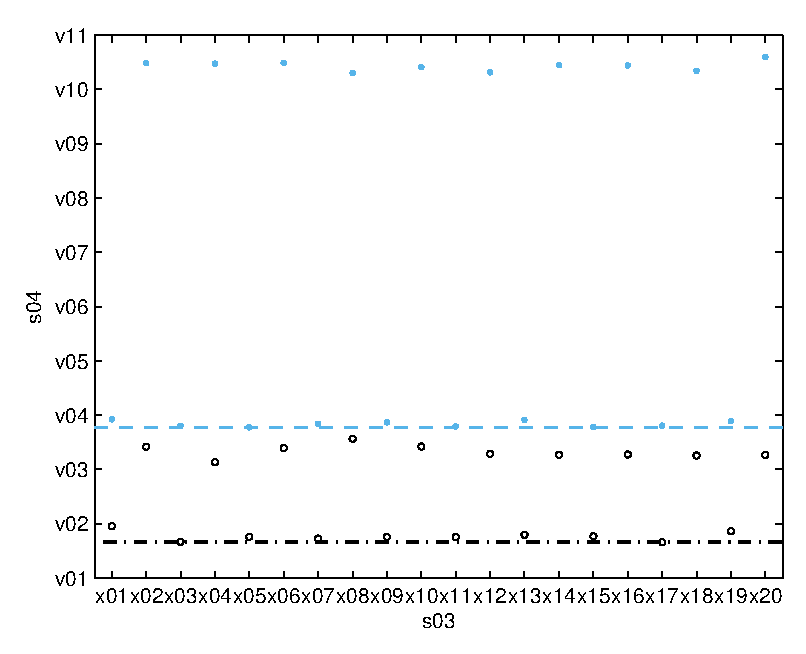
\includegraphics{bias_sigma_1_85.eps}}%
\end{psfrags}%
%
% End bias_sigma_1_85.tex
\end{document}
% See http://www.mathworks.de/matlabcentral/fileexchange/loadFile.do?objectId=4638
% for recent versions of laprint.m.
%
% created by:           LaPrint version 3.16 (13.9.2004)
% created on:           16-Jul-2013 16:48:36
% eps bounding box:     15 cm x 11.25 cm
% comment:              
%
\begin{psfrags}%
\psfragscanon%
%
% text strings:
\psfrag{s03}[t][t]{\color[rgb]{0,0,0}\setlength{\tabcolsep}{0pt}\begin{tabular}{c}{\Large{}Calculation number}\end{tabular}}%
\psfrag{s04}[b][b]{\color[rgb]{0,0,0}\setlength{\tabcolsep}{0pt}\begin{tabular}{c}{\Large$\log \sigma_1$}\end{tabular}}%
%
% xticklabels:
\psfrag{x01}[t][t]{1}%
\psfrag{x02}[t][t]{2}%
\psfrag{x03}[t][t]{3}%
\psfrag{x04}[t][t]{4}%
\psfrag{x05}[t][t]{5}%
\psfrag{x06}[t][t]{6}%
\psfrag{x07}[t][t]{7}%
\psfrag{x08}[t][t]{8}%
\psfrag{x09}[t][t]{9}%
\psfrag{x10}[t][t]{10}%
\psfrag{x11}[t][t]{11}%
\psfrag{x12}[t][t]{12}%
\psfrag{x13}[t][t]{13}%
\psfrag{x14}[t][t]{14}%
\psfrag{x15}[t][t]{15}%
\psfrag{x16}[t][t]{16}%
\psfrag{x17}[t][t]{17}%
\psfrag{x18}[t][t]{18}%
\psfrag{x19}[t][t]{19}%
\psfrag{x20}[t][t]{20}%
%
% yticklabels:
\psfrag{v01}[r][r]{-5.9}%
\psfrag{v02}[r][r]{-5.8}%
\psfrag{v03}[r][r]{-5.7}%
\psfrag{v04}[r][r]{-5.6}%
\psfrag{v05}[r][r]{-5.5}%
\psfrag{v06}[r][r]{-5.4}%
\psfrag{v07}[r][r]{-5.3}%
\psfrag{v08}[r][r]{-5.2}%
\psfrag{v09}[r][r]{-5.1}%
\psfrag{v10}[r][r]{-5}%
\psfrag{v11}[r][r]{-4.9}%
%
% Figure:
\resizebox{12cm}{!}{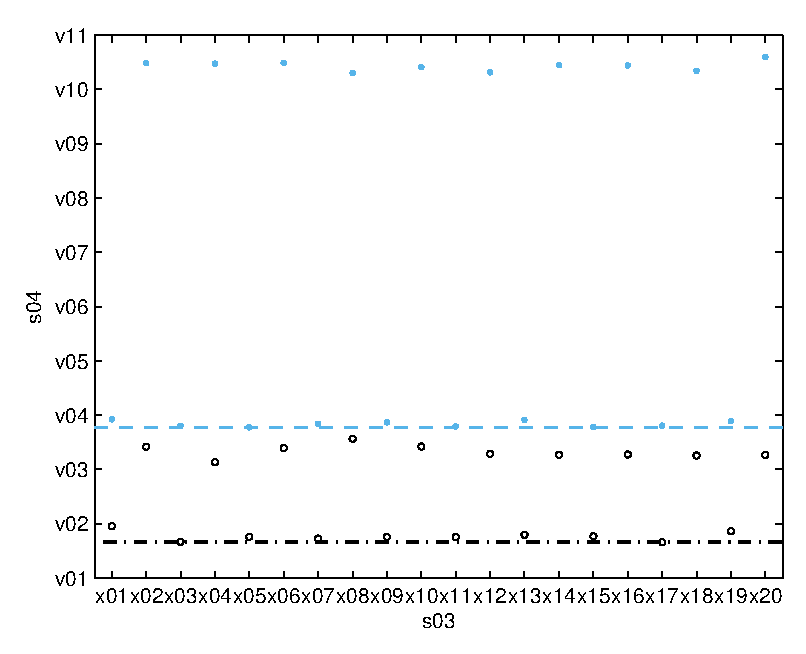
\includegraphics{bias_sigma_1_85.eps}}%
\end{psfrags}%
%
% End bias_sigma_1_85.tex
\end{document}
% See http://www.mathworks.de/matlabcentral/fileexchange/loadFile.do?objectId=4638
% for recent versions of laprint.m.
%
% created by:           LaPrint version 3.16 (13.9.2004)
% created on:           16-Jul-2013 13:44:05
% eps bounding box:     15 cm x 11.25 cm
% comment:              
%
\begin{psfrags}%
\psfragscanon%
%
% text strings:
\psfrag{s03}[t][t]{\color[rgb]{0,0,0}\setlength{\tabcolsep}{0pt}\begin{tabular}{c}{\Large{}Calculation number}\end{tabular}}%
\psfrag{s04}[b][b]{\color[rgb]{0,0,0}\setlength{\tabcolsep}{0pt}\begin{tabular}{c}{\Large$\log \sigma_{\ln(M_\bullet/M_\odot)}$}\end{tabular}}%
%
% xticklabels:
\psfrag{x01}[t][t]{$1$}%
\psfrag{x02}[t][t]{$2$}%
\psfrag{x03}[t][t]{$3$}%
\psfrag{x04}[t][t]{$4$}%
\psfrag{x05}[t][t]{$5$}%
\psfrag{x06}[t][t]{$6$}%
\psfrag{x07}[t][t]{$7$}%
\psfrag{x08}[t][t]{$8$}%
\psfrag{x09}[t][t]{$9$}%
\psfrag{x10}[t][t]{$10$}%
\psfrag{x11}[t][t]{$11$}%
\psfrag{x12}[t][t]{$12$}%
\psfrag{x13}[t][t]{$13$}%
\psfrag{x14}[t][t]{$14$}%
\psfrag{x15}[t][t]{$15$}%
\psfrag{x16}[t][t]{$16$}%
\psfrag{x17}[t][t]{$17$}%
\psfrag{x18}[t][t]{$18$}%
\psfrag{x19}[t][t]{$19$}%
\psfrag{x20}[t][t]{$20$}%
%
% yticklabels:
\psfrag{v01}[r][r]{$-5.9$}%
\psfrag{v02}[r][r]{$-5.8$}%
\psfrag{v03}[r][r]{$-5.7$}%
\psfrag{v04}[r][r]{$-5.6$}%
\psfrag{v05}[r][r]{$-5.5$}%
\psfrag{v06}[r][r]{$-5.4$}%
\psfrag{v07}[r][r]{$-5.3$}%
\psfrag{v08}[r][r]{$-5.2$}%
\psfrag{v09}[r][r]{$-5.1$}%
\psfrag{v10}[r][r]{$-5.0$}%
\psfrag{v11}[r][r]{$-4.9$}%
%
% Figure:
\resizebox{12cm}{!}{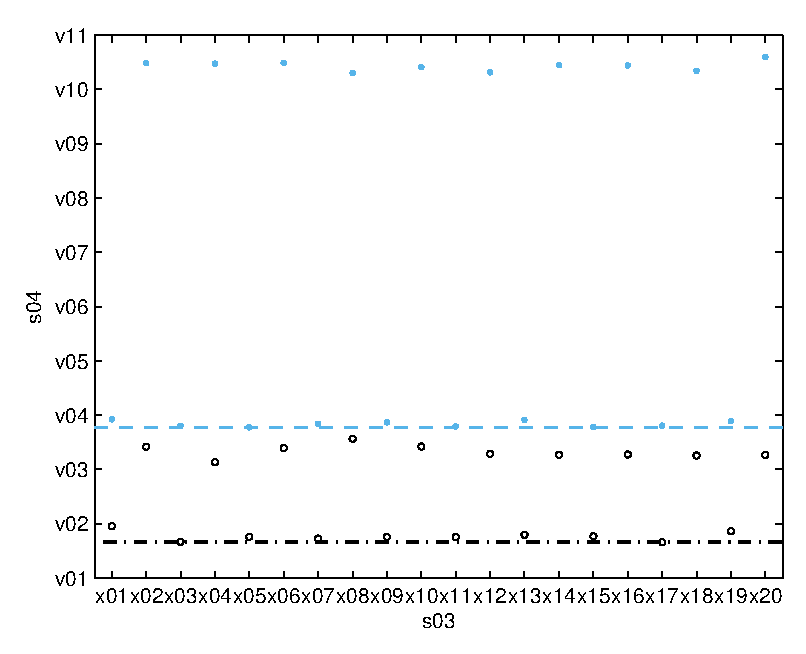
\includegraphics{bias_sigma_1_85.eps}}%
\end{psfrags}%
%
% End bias_sigma_1_85.tex
